%=========================================================

% Here you can choose to compile with or without solutions.
% However, this definition is ignored if you use any
% command from the `Makefile`.
\providecommand{\withSol}{\iftrue}

%=========================================================

\documentclass
[twoside,english,colorbacktitle,accentcolor=tud9c]
{tudexercise}

\usepackage[T1]{fontenc}
\usepackage[latin9]{inputenc}
\usepackage{amstext}
\usepackage{amsmath}
\usepackage{graphicx}
\usepackage{setspace}
\usepackage{multicol}
\usepackage{mathtools}
\usepackage{dsfont}
\usepackage{units}
\usepackage{subfigure}
\usepackage{color}
\usepackage{booktabs}
\usepackage{fancyref}
\usepackage[ngerman,english]{babel}

\usepackage{pdfpages}

%=========================================================

\def\homework{3}
\def\homeworkVer{1}
\def\homeworkSolVer{1}

%=========================================================

\ifcsname withSol\endcsname\else
  \expandafter\let\csname withSol\expandafter\endcsname
                  \csname iffalse\endcsname
\fi

\withSol
	\usepackage[solutions]{iasHomework}
\else
	\usepackage{iasHomework}
\fi

%=========================================================

\hwtitle{Robot Learning}
{Winter Semester 2016}
{Prof. Dr. J. Peters, F. Veiga, S. Parisi}

\begin{document}

%=========================================================

\maketitle

\begin{examheader}
	\textmb{Robot Learning - Homework \arabic{section}}
	\examheaderdefault 
\end{examheader} 

\deadline{Tuesday, 31 January 2017 (3 pm)}

%=========================================================

\exercise{Optimal Control}
In this exercise, we consider a finite-horizon discrete time-varying Stochastic Linear Quadratic Regulator with Gaussian noise and time-varying quadratic reward function. Such system is defined as
%
\begin{align}
	\vec s_{t+1} = \mat A_t \vec s_t + \mat B_t \vec a_t + \vec w_t\,, 
\end{align}
where $\vec s_t$ is the state, $\vec a_t$ is the control signal, $\vec w_t \sim \gauss{\vec b_t}{\Sigma_t}$ is Gaussian additive noise with mean $\vec b_t$ and covariance $\Sigma_t$ and $t=0,1,\dots,T$ is the time horizon. 
The control signal $\vec a_t$ is computed as
%
\begin{align}
	\vec a_t = - \mat K_t \vec s_t + \vec k_t
\end{align}
%
and the reward function $r_t$ is
%
\begin{align}
	r_t = \begin{cases}
	- (\vec s_t - \vec r_t)\T \mat R_t (\vec s_t - \vec r_t) - \vec a\T_t \mat H_t \vec a_t  & \text{when \quad} t=0,1,\dots,T-1
	\\
	- (\vec s_t - \vec r_t)\T \mat R_t (\vec s_t - \vec r_t) & \text{when \quad} t=T
	\end{cases}
\end{align}
	
\textbf{Note: $r_t$ and $\vec r_t$ are different!}

\textbf{Note 2: the notation used in Marc Toussaint's notes ``\textit{(Stochastic) Optimal Control''} is different from the one used in the lecture's slides.}	
	
\begin{questions}

%----------------------------------------------

\begin{question}{Implementation}{8}
	Implement the LQR with the following properties
	\begin{align*}
	\vec s_0 & \sim \gauss{0}{1} &	T &= 50
	\\
	\mat A_t &= \begin{bmatrix}
       1 & 0.1\\
       0 & 1
    \end{bmatrix} &
	\mat B_t &= \begin{bmatrix}
       0 \\
       0.1
    \end{bmatrix}
    \\
	\vec b_t &= \begin{bmatrix}
       5\\
       0
    \end{bmatrix} & \Sigma_t &= 0.01
	\\
	\mat K_t &= \begin{bmatrix}
       5 &
       0.3
    \end{bmatrix} & 
	\vec k_t &= 0.3 & 
	\\
	\mat H_t &= 1 & 		
	\mat R_t &= \begin{cases}
	\begin{bmatrix}
	100000 &0\\
	0&0.1
	\end{bmatrix}  & \text{if \quad} t=14, 40
	\\
	\begin{bmatrix}
	0.01 &0\\
	0&0.1
	\end{bmatrix} & \text{otherwise}
	\end{cases}	
	&
	\vec r_t &= \begin{cases}
	\begin{bmatrix}
	10\\
	0
	\end{bmatrix}  & \text{if \quad} t=0,1,\ldots,14
	\\
	\begin{bmatrix}
	20\\
	0
	\end{bmatrix}  & \text{if \quad} t=15,16,\ldots,T
	\end{cases}	
	\end{align*}
	
	Execute the system 20 times.
	Plot the mean and 95\% confidence over the different experiments of the state $\vec s_t$ and of the control signal $\vec a_t$ over time. 
	How does the system behave? 
	Compute and write down the mean and the standard deviation of the cumulative reward over the experiments. 
	Attach a snippet of your code.
	
\begin{answer}
The system is following a spiral trajectory. The actual variance cant be shown with the plt plot function, because its a Tube around the red line with the height of the walls and just touching the walls in the middle.\\
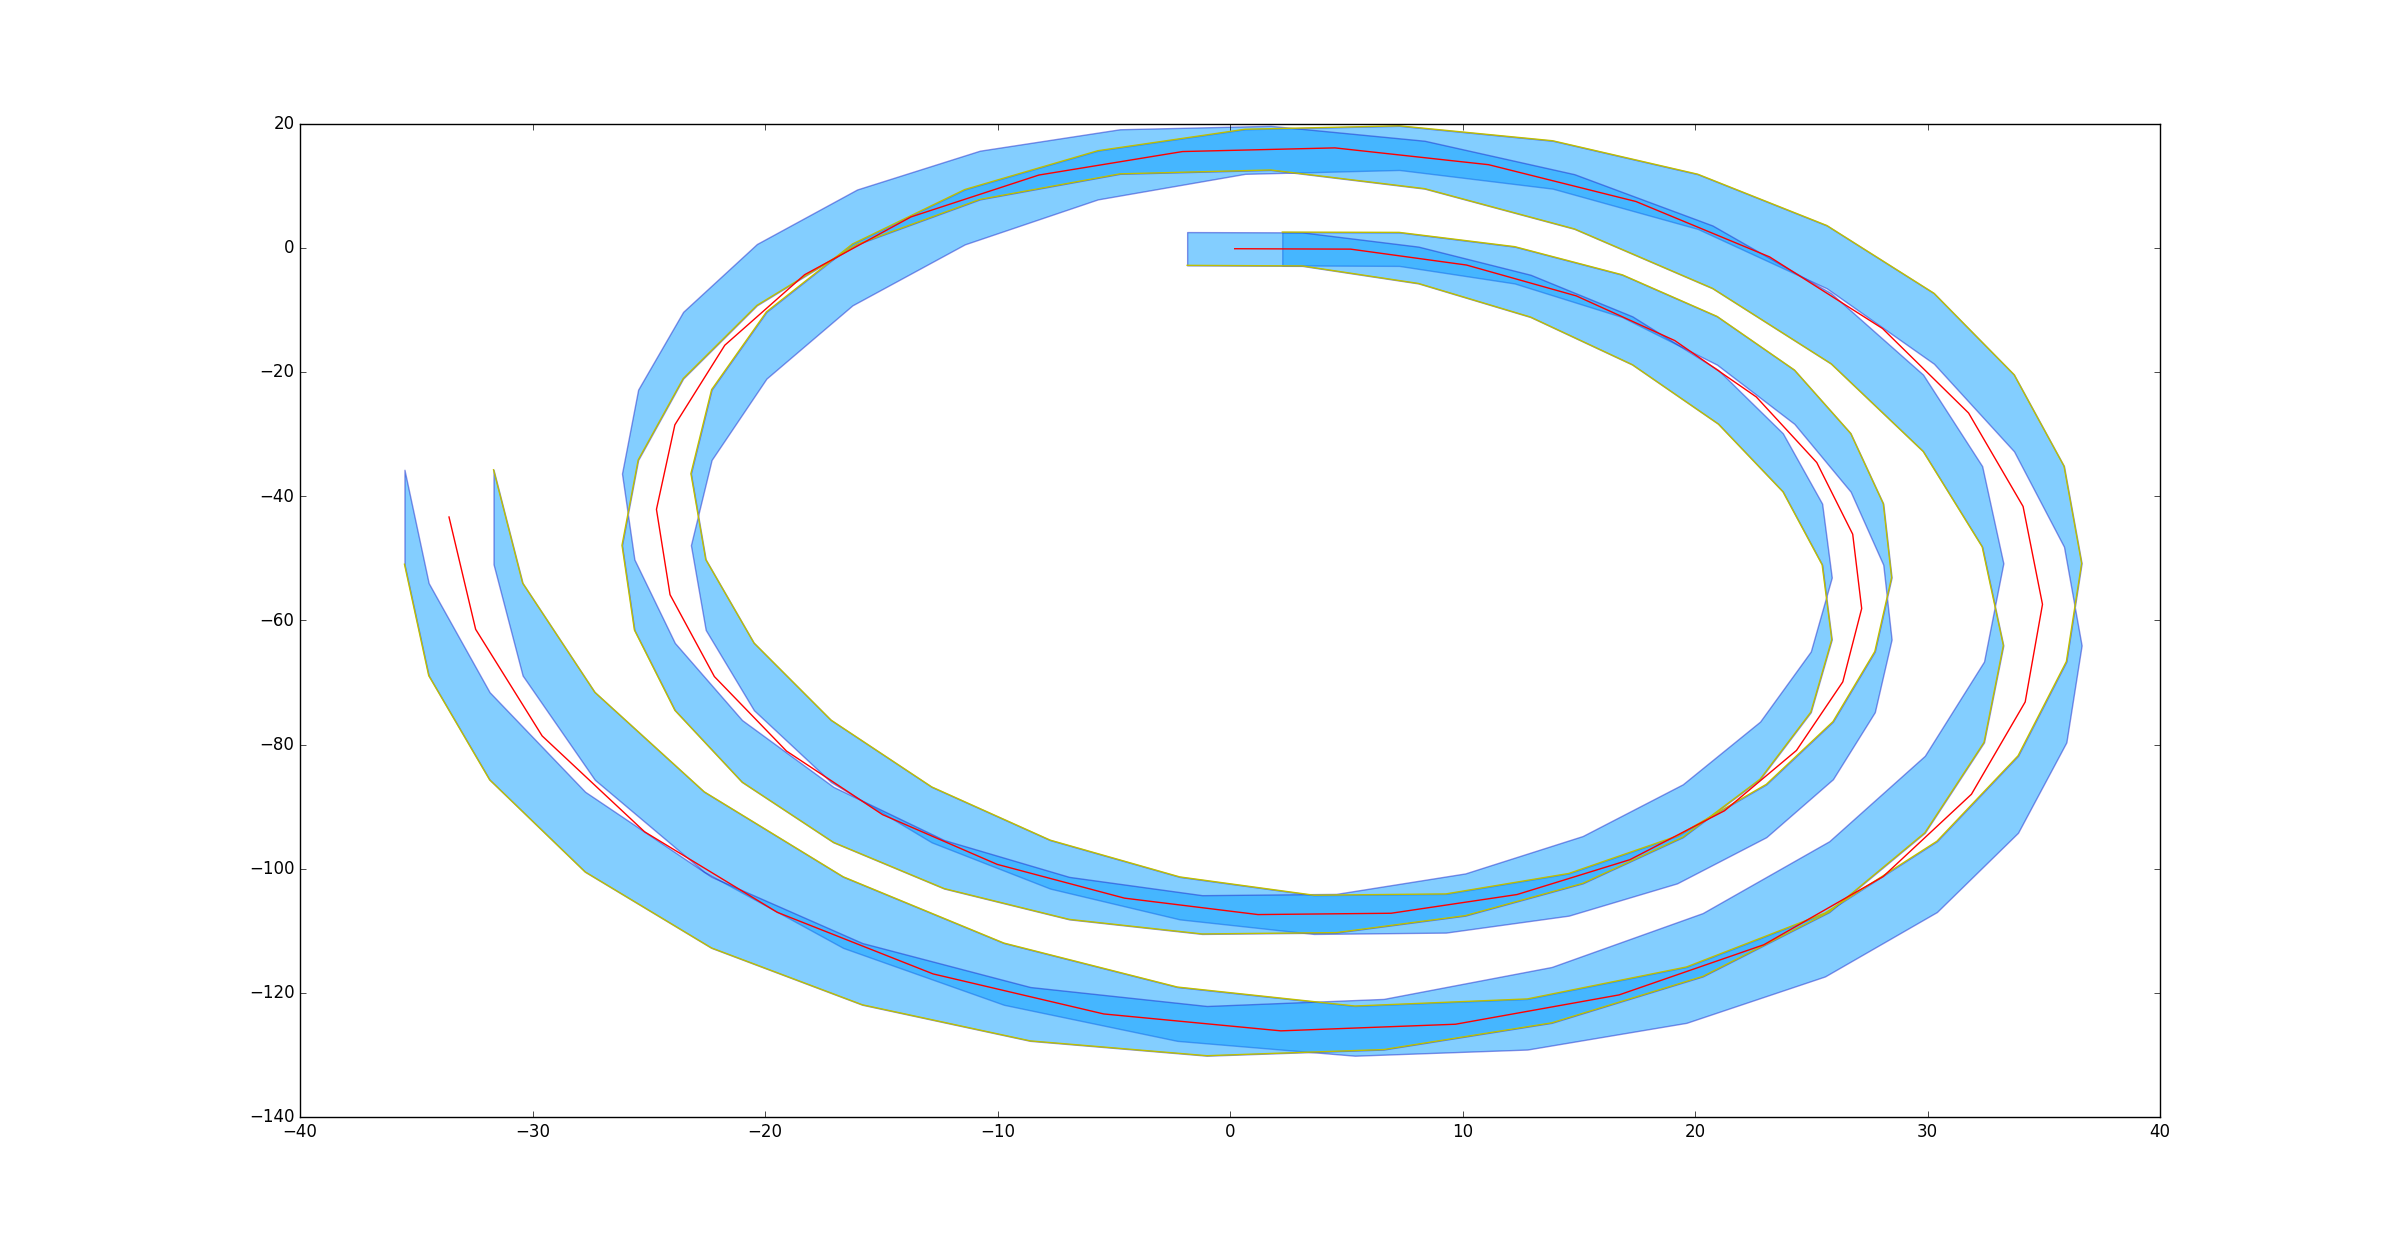
\includegraphics[scale=0.35,trim=70mm 0mm 0mm 0mm,clip=true]{states_a.png}
The Actions are oscillating as aspected for such an spiral trajectory.\\
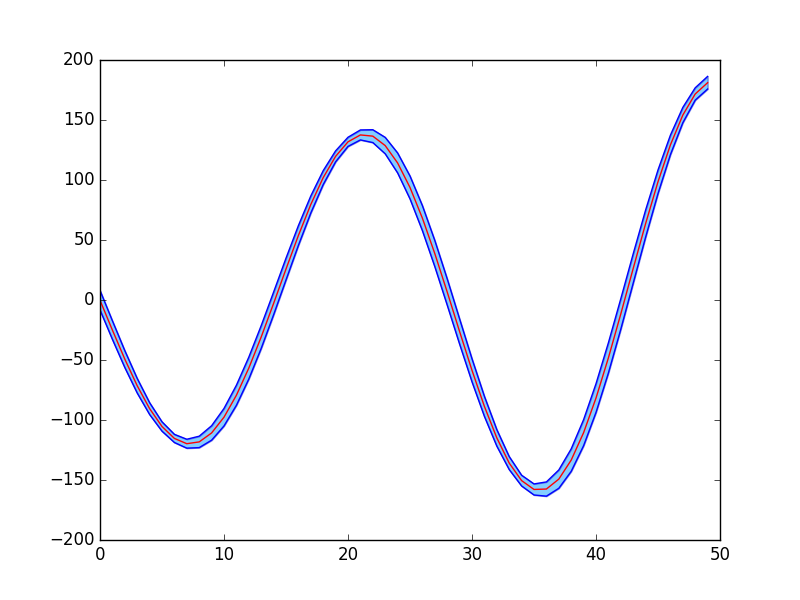
\includegraphics[scale=0.35,trim=70mm 0mm 0mm 0mm,clip=true]{actions_a.png}
\newpage
negative cumulative reward:\\
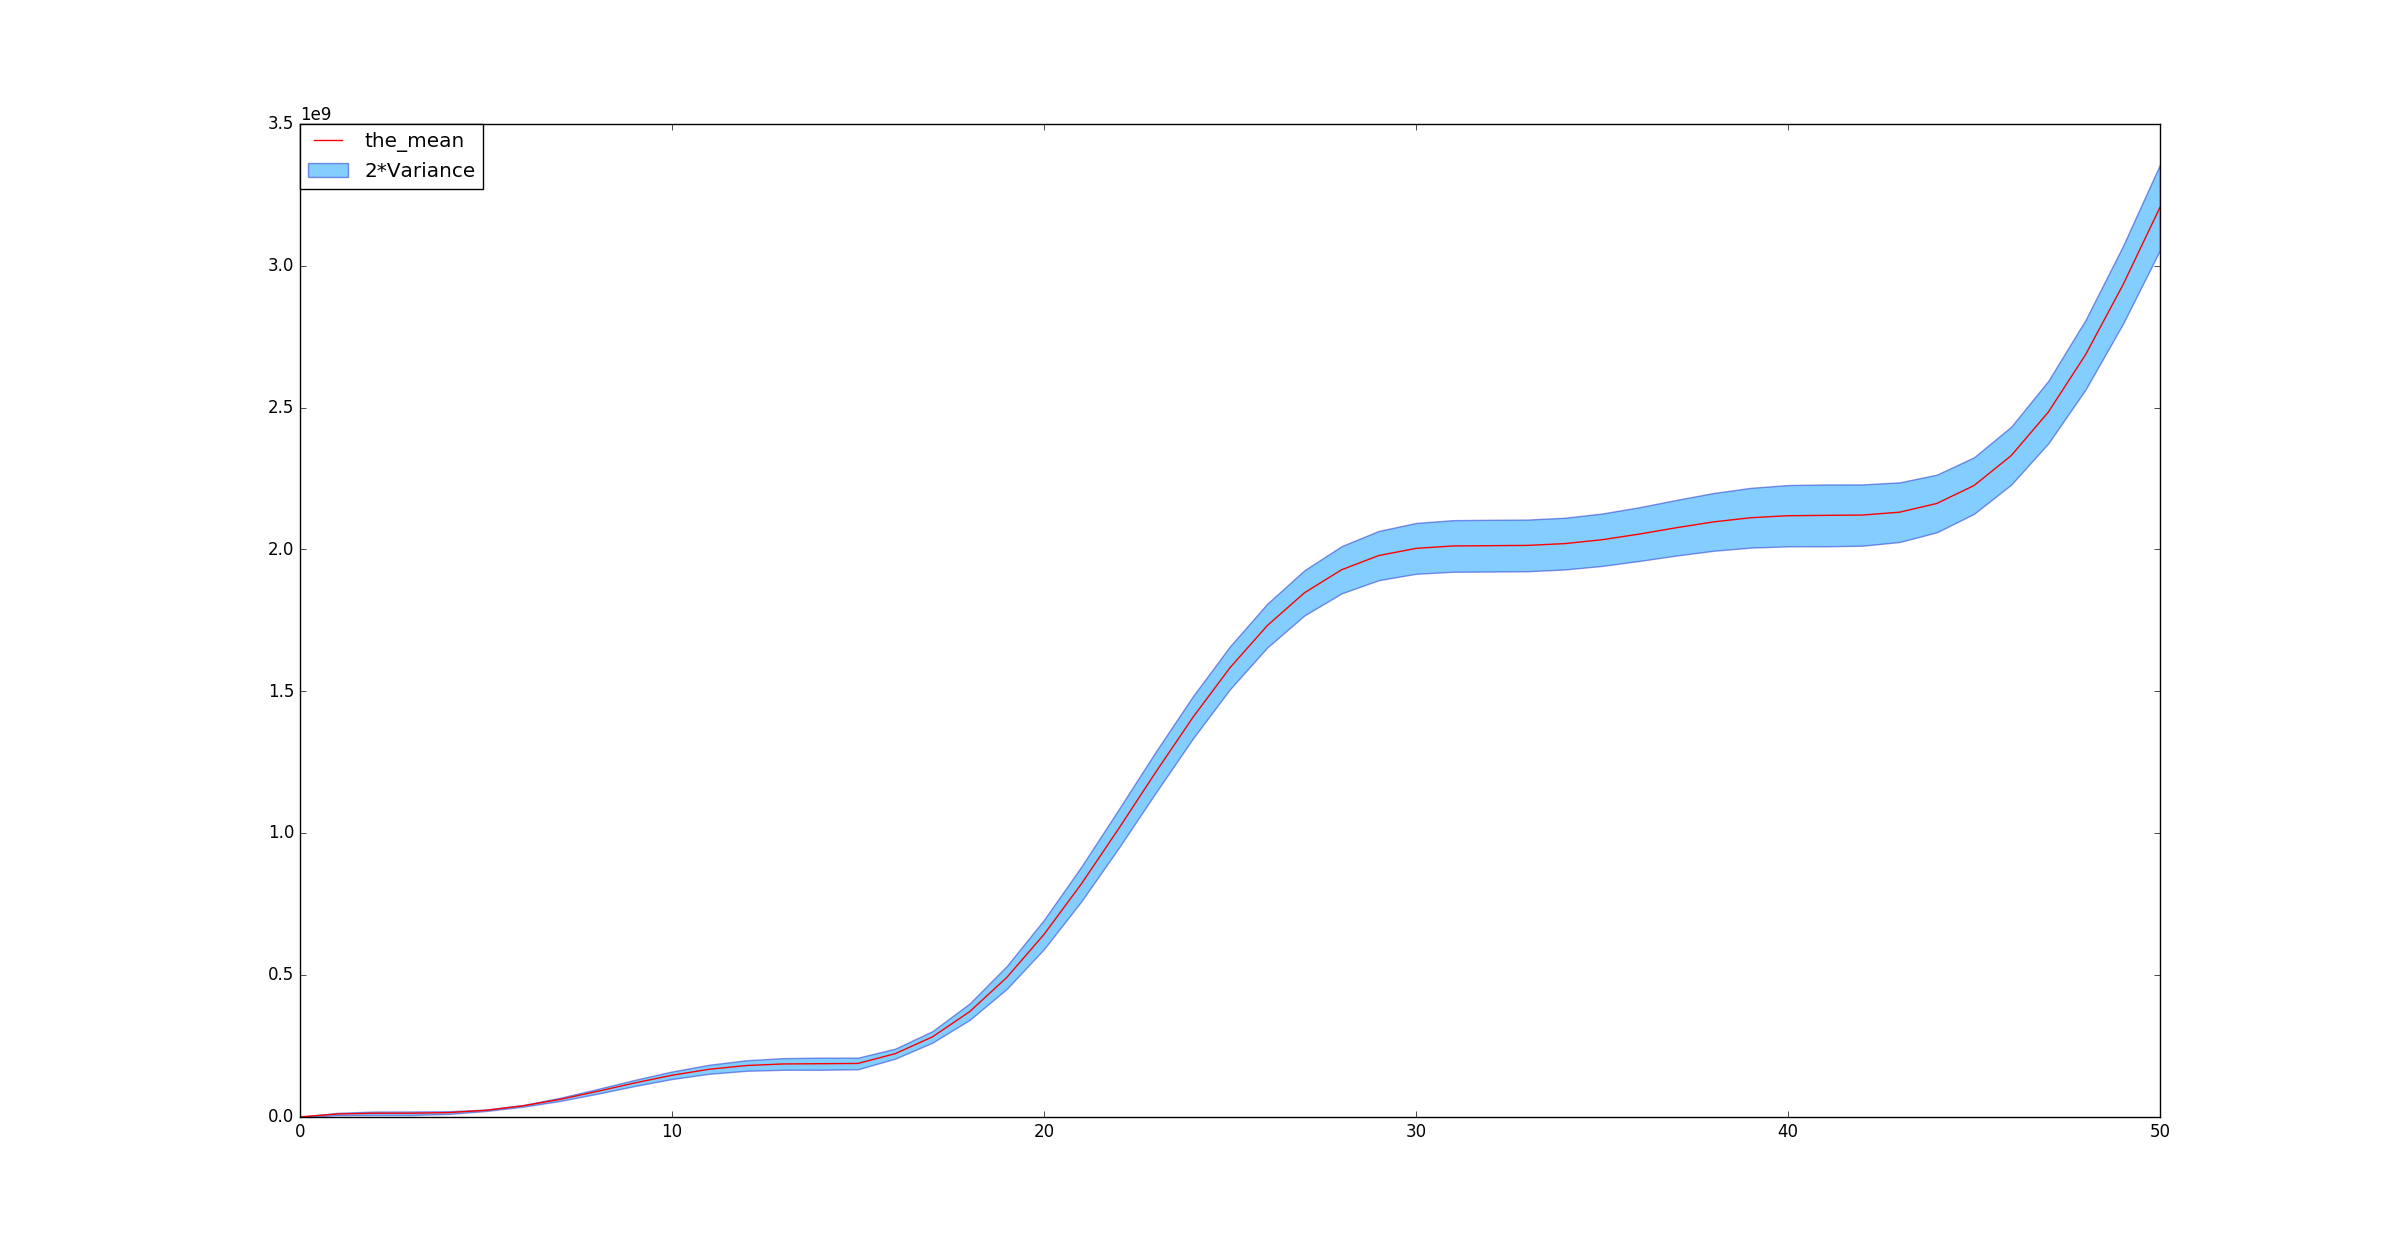
\includegraphics[scale=0.35,trim=70mm 0mm 0mm 0mm,clip=true]{rewards_a.png}
\newpage
\lstinputlisting[language=Python,breaklines=true]{lqr-1a.py}
\end{answer}


\end{question}

%---------------------------------

\begin{question}{LQR as a P controller}{4}

	The LQR can also be seen as a simple P controller of the form
	%
	\begin{align}
		\vec a_t = \mat K_t (\vec s^\text{des}_t - \vec s_t) + \vec k_t\,,
	\end{align}
	%
	which corresponds to the controller used in the canonical LQR system with the introduction of the target $\vec s^\text{des}_t$.
	
	Assume as target 
	\begin{align}
        \vec s^\text{des}_t = \vec r_t = \begin{cases}
        \begin{bmatrix}
        10\\
        0
        \end{bmatrix}  & \text{if \quad} t=0,1,\ldots,14
        \\
        \begin{bmatrix}
        20\\
        0
        \end{bmatrix}  & \text{if \quad} t=15,16,\ldots,T
        \end{cases}	
	\end{align}
    
    Use the same LQR system as in the previous exercise and run 20 experiments. Plot in one figure the mean and 95\% confidence of the first state, for both $\vec s^\text{des}_t = \vec r_t$ and $\vec s^\text{des}_t = \vec 0$.

\begin{answer}
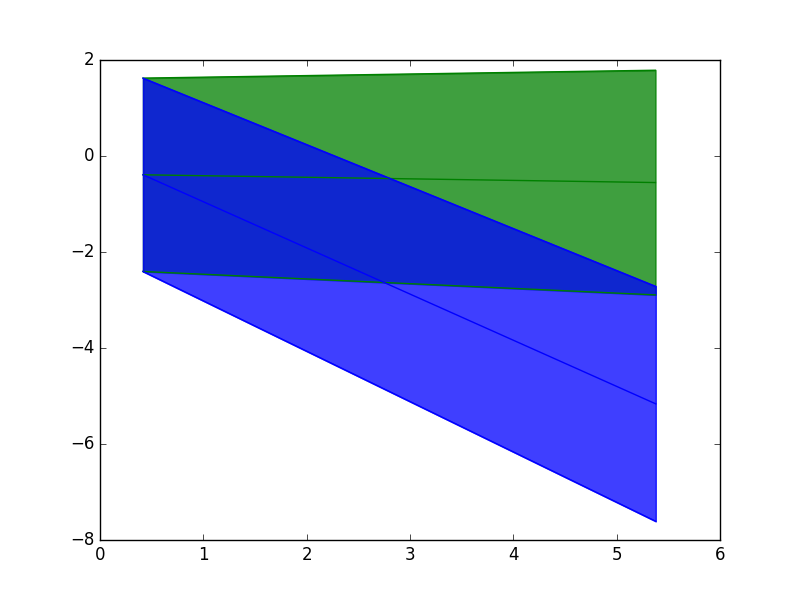
\includegraphics[scale=0.35,trim=0mm 0mm 0mm 0mm,clip=true]{states_b.png}
\end{answer}
\end{question}

%---------------------------------
	
	
\begin{question}{Optimal LQR}{8}
	To compute the optimal gains $\mat K_t$ and $\vec k_t$, which maximize the cumulative reward, we can use an analytic optimal solution. This controller recursively computes the optimal action by
	\begin{align}
		\vec a^* &= -(\mat H_t + \mat B^T_t \mat V_{t+1}\mat B_t)^{-1}	\mat B^T_t (\mat V_{t+1} (\mat A_t \vec s_t+\mat b_t )- \vec v_{t+1} ),
	\end{align}
	which can be decomposed into
	\begin{align}
		\mat K_t &= -(\mat H_t + \mat B^T_t \mat V_{t+1}\mat B_t)^{-1}	\mat B^T_t \mat V_{t+1} \mat A_t,
		\\
		\mat k_t &= -(\mat H_t + \mat B^T_t \mat V_{t+1}\mat B_t)^{-1}	\mat B^T_t (\mat V_{t+1} \mat b_t - \vec v_{t+1}).
	\end{align}
	%
	where
	%
	\begin{align}
		\mat M_t &= \mat B_t(\mat H_t + \mat B^T_t \mat V_{t+1}\mat B_t)^{-1}	\mat B^T_t \mat V_{t+1} \mat A_t
		\\
		\mat V_t &=
		\begin{cases}
	       \mat R_t + (\mat A_t - \mat M_t)^T\mat V_{t+1}\mat A_t & \text{when \quad} t = 1...T-1
	       \\
	       \mat R_t & \text{when \quad} t = T
	    \end{cases}
	    \\
		\mat v_t &= 
		\begin{cases}
	       \mat R_t\vec r_t + (\mat A_t - \mat M_t)^T(\vec v_{t+1} - \mat V_{t+1}\mat b_t) & \text{when \quad} t = 1...T-1
	       \\
	       \mat R_t\vec r_t & \text{when \quad} t = T
	    \end{cases}
	\end{align}		 

	Run 20 experiments with $\vec s^\text{des}_t = \vec 0$ computing the optimal gains $\mat K_t$ and $\vec k_t$. Plot the mean and 95\% confidence of both states for all three different controllers used so far. Use one figure per state. 
	Report the mean and std of the cumulative reward for each controller and comment the results. Attach a snippet of your code.

\begin{answer}
The contoller of 1c) has a much higher Variance than the others.\\
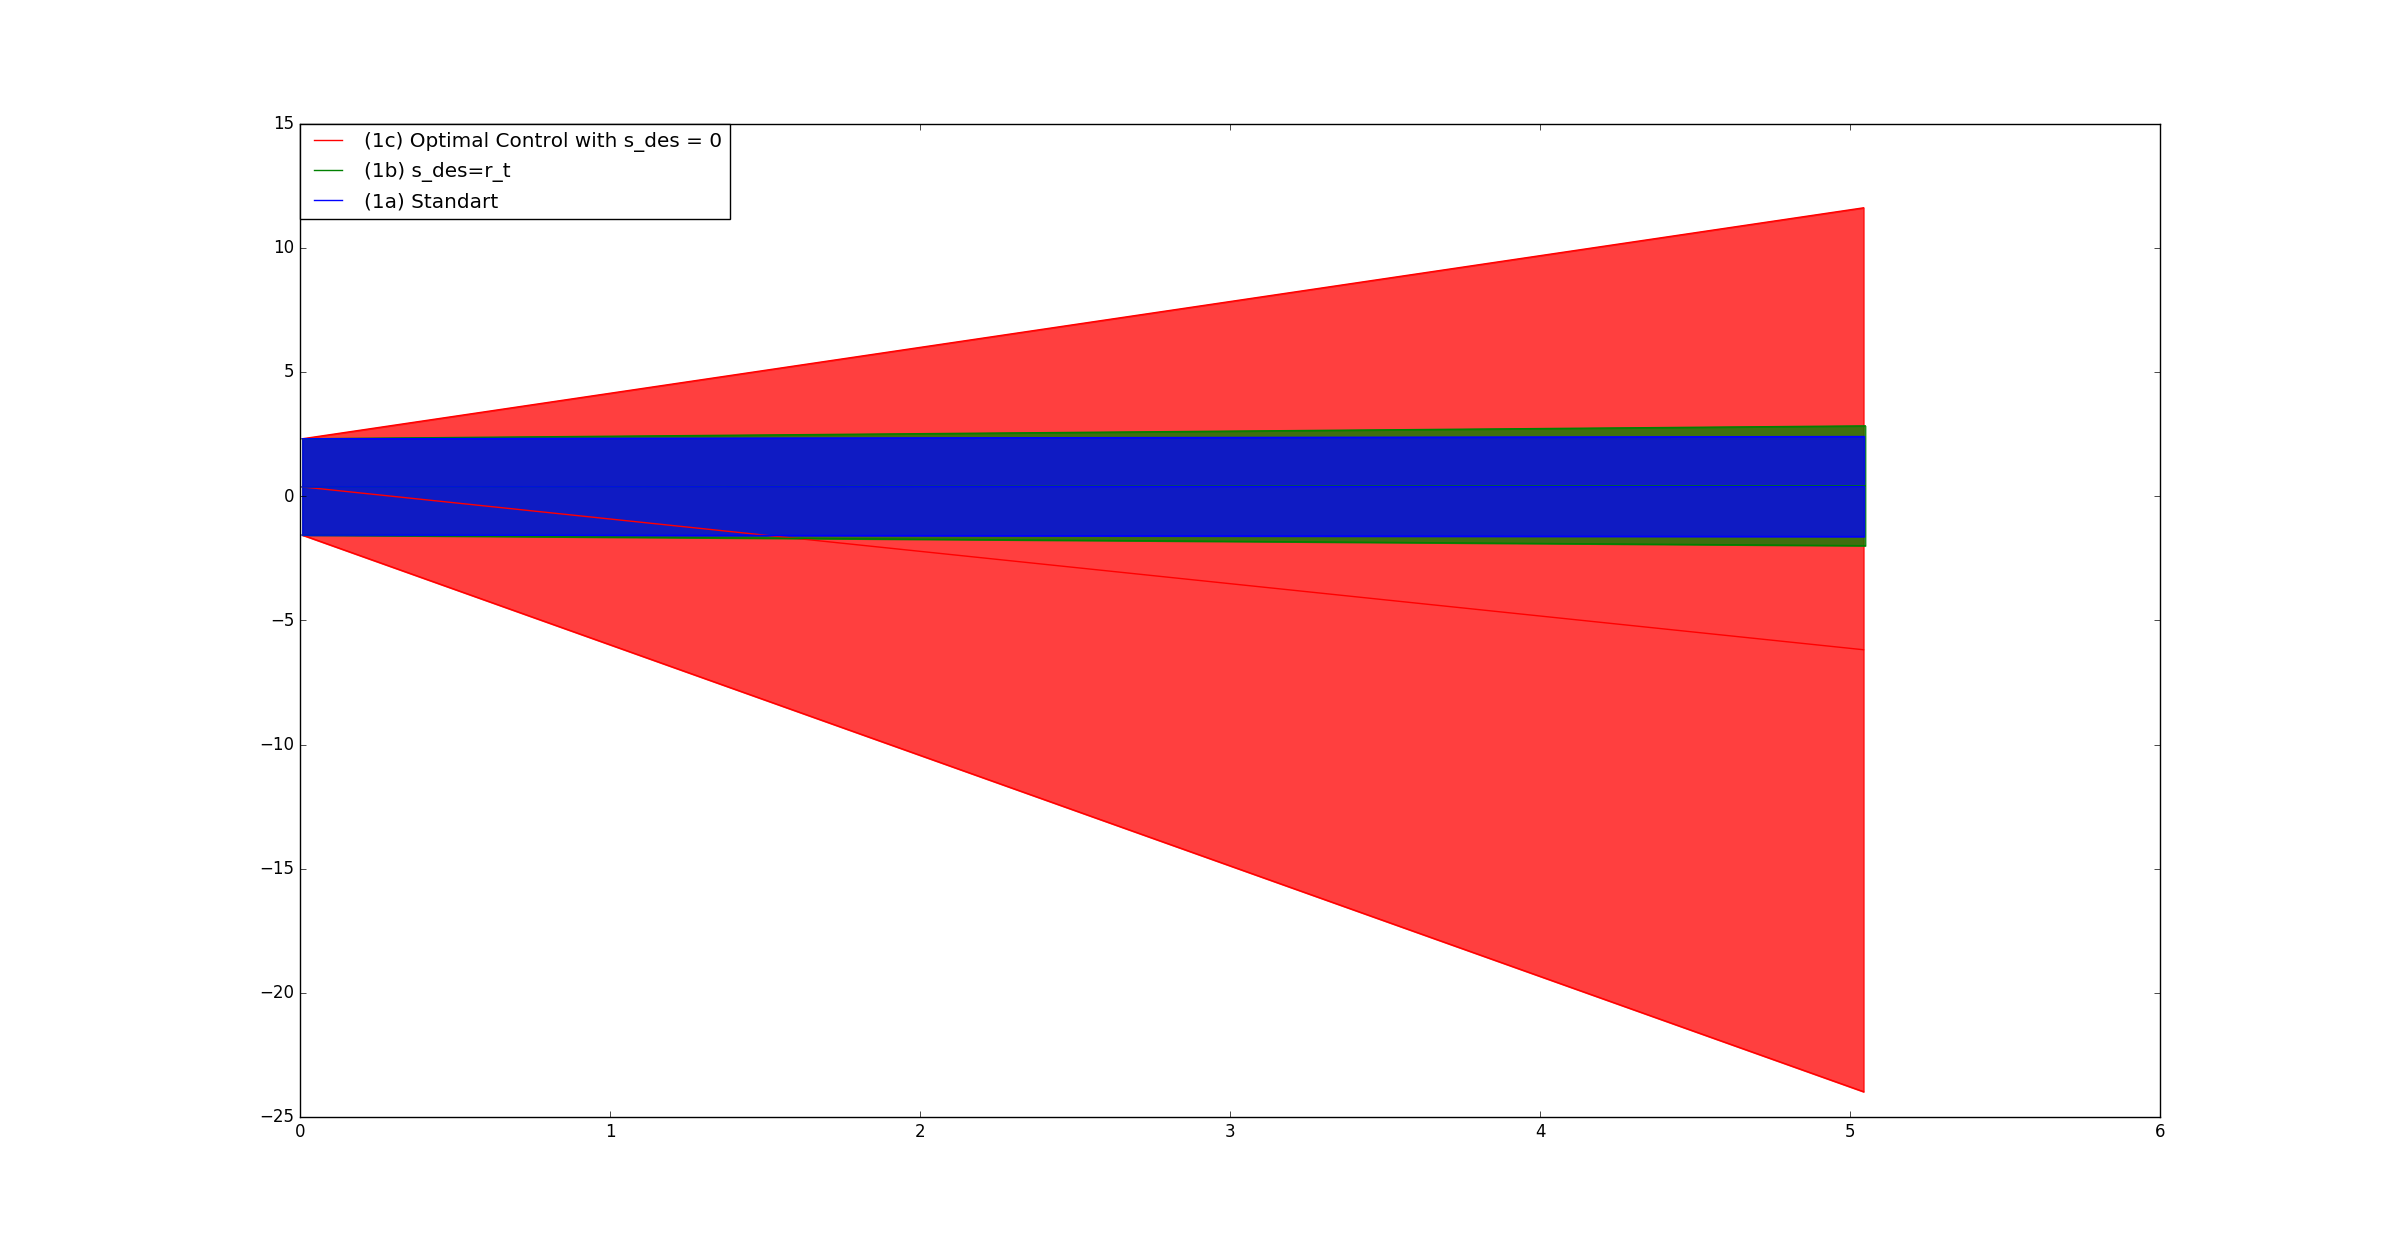
\includegraphics[scale=0.35,trim=70mm 0mm 0mm 0mm,clip=true]{states_c2.png}
As you can see rewards for 1c) are way too big, therefore we plot 1a) and 1b) together again (voilet = red+ blue)\\
negative cumulative reward:\\
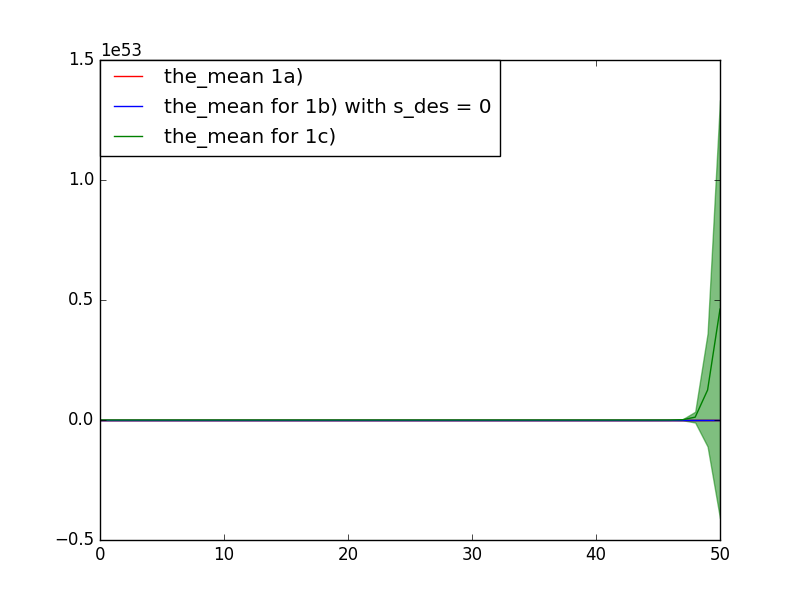
\includegraphics[scale=0.35,trim=0mm 0mm 0mm 0mm,clip=true]{rewards_c.png}
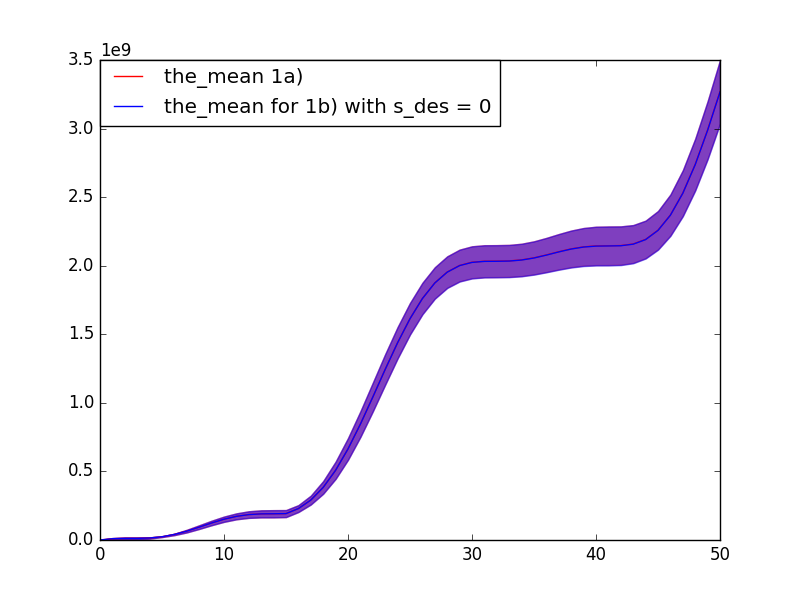
\includegraphics[scale=0.35,trim=0mm 0mm 0mm 0mm,clip=true]{rewards_c2.png}\newpage
\lstinputlisting[language=Python,breaklines=true]{lqr-1a.py}
\end{answer}

\end{question}

%----------------------------------------------

\end{questions}



\newif\ifvimbug
\vimbugfalse

\ifvimbug
\begin{document}
\fi

\exercise{Reinforcement Learning}

You recently acquired a robot for cleaning you apartment but you are not happy with its performance and you decide to reprogram it using the latest AI algorithms. As a consequence the robot became self-aware and, whenever you are away, it prefers to play with toys rather than cleaning the apartment. Only the cat has noticed the strange behavior and attacks the robot. The robot is about to start its day and its current perception of the environment is as following 
%
\begin{center}
	%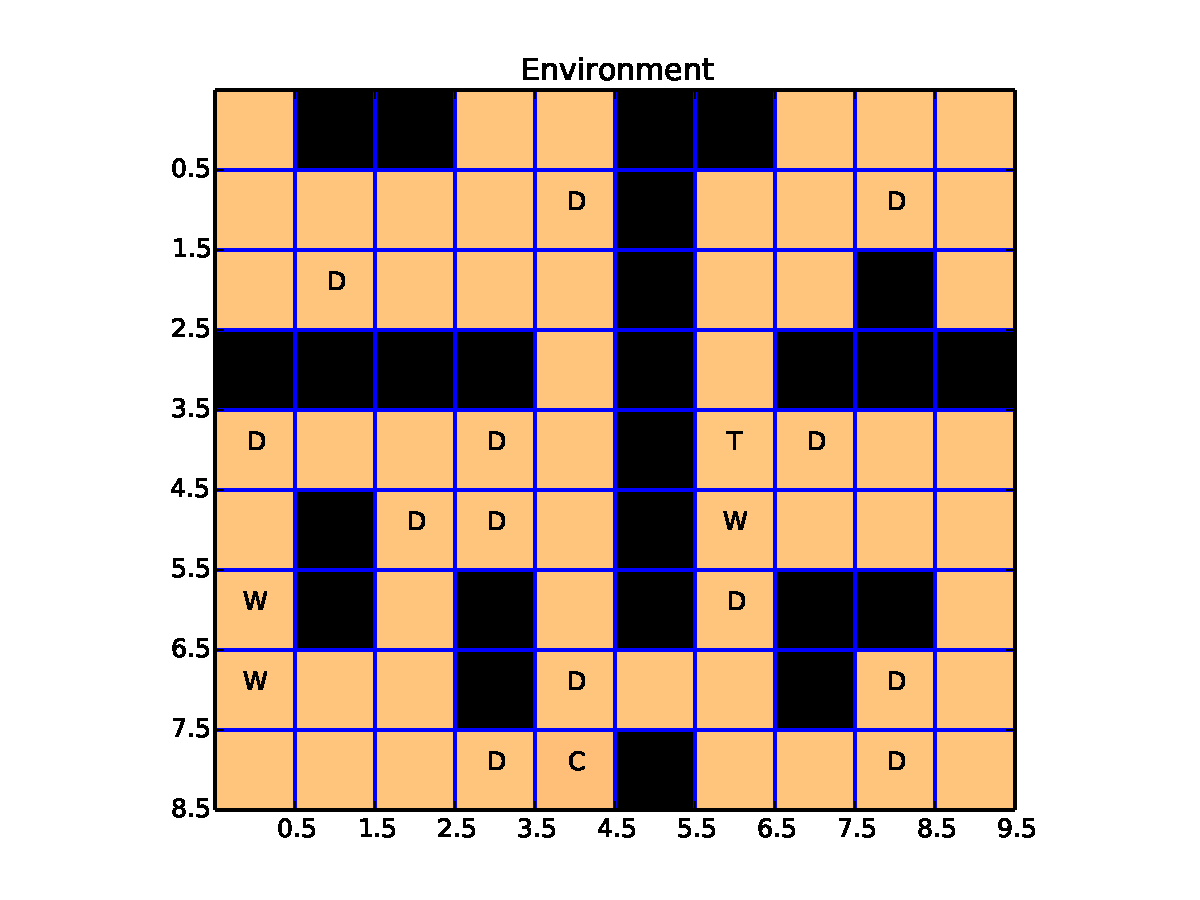
\includegraphics[width=0.75\textwidth]{fig/gridworld.pdf}
	\colorbox{yellow}{Your graphic could be here. It just wasn't included.}
\end{center}
%
The black squares denote extremely dangerous states that the robot must avoid to protect its valuable sensors. The reward of such states is set to $r_\textrm{danger}=-10^5$ (NB: the robot can still go through these states!). Moreover, despite being waterproof, the robot developed a phobia of water (W), imitating the cat. The reward of states with water is $r_\textrm{water}=-100$. The robot is also afraid of the cat (C) and tries to avoid it at any cost. The reward when encountering the cat is $r_\textrm{cat}=-3000$. The state containing the toy (T) has a reward of $r_\textrm{toy}=1000$, as the robot enjoys playing with them. Some of the initial specification still remain, therefore the robot receives $r_\textrm{dirt}=35$ in states with dirt (D).

State rewards can be collected at every time the robot is at that state. 
The robot can perform the following actions: \textit{down, right, up, left} and
\textit{stay}.

In our system we represent the actions with the an ID (0, 1, 2, 3, 4), while the grid is indexed as $\{ \texttt{row}, \texttt{column} \}$. The robot can't leave the grid as it is surrounded with walls.
A skeleton of the gridworld code and some plotting functions are available at the webpage.
For all the following questions, always attach a snippet of your code.


\begin{questions}

\begin{question}{Finite Horizon Problem}{14}
In the first exercise we consider the finite horizon problem, with horizon $T=15$ steps.
The goal of the robot is to maximize the expected return 
\begin{equation}
J_\pi = \mathbb{E}_\pi\left[\sum_{t=1}^{T-1}r_t(s_t,a_t)+r_T(s_T)\right], \label{Eq:J}
\end{equation}
according to policy $\pi$, state $s$, action $a$, reward $r$, and horizon $T$. Since rewards in our case are independent of the action and the actions are deterministic, Equation~\eqref{Eq:J} becomes
\begin{equation}
J_\pi = \sum_{t=1}^{T}r_t(s_t).
\end{equation}
Using the Value Iteration algorithm, determine the optimal action for each state when the robot has 15 steps left. Attach the plot of the policy to your answer and a mesh plot for the value function. Describe and comment the policy: is the robot avoiding the cat and the water? Is it collecting dirt and playing with the toy? Which would be the time horizon that makes the robot acts differently in state $(9,4)$?

\begin{answer}
	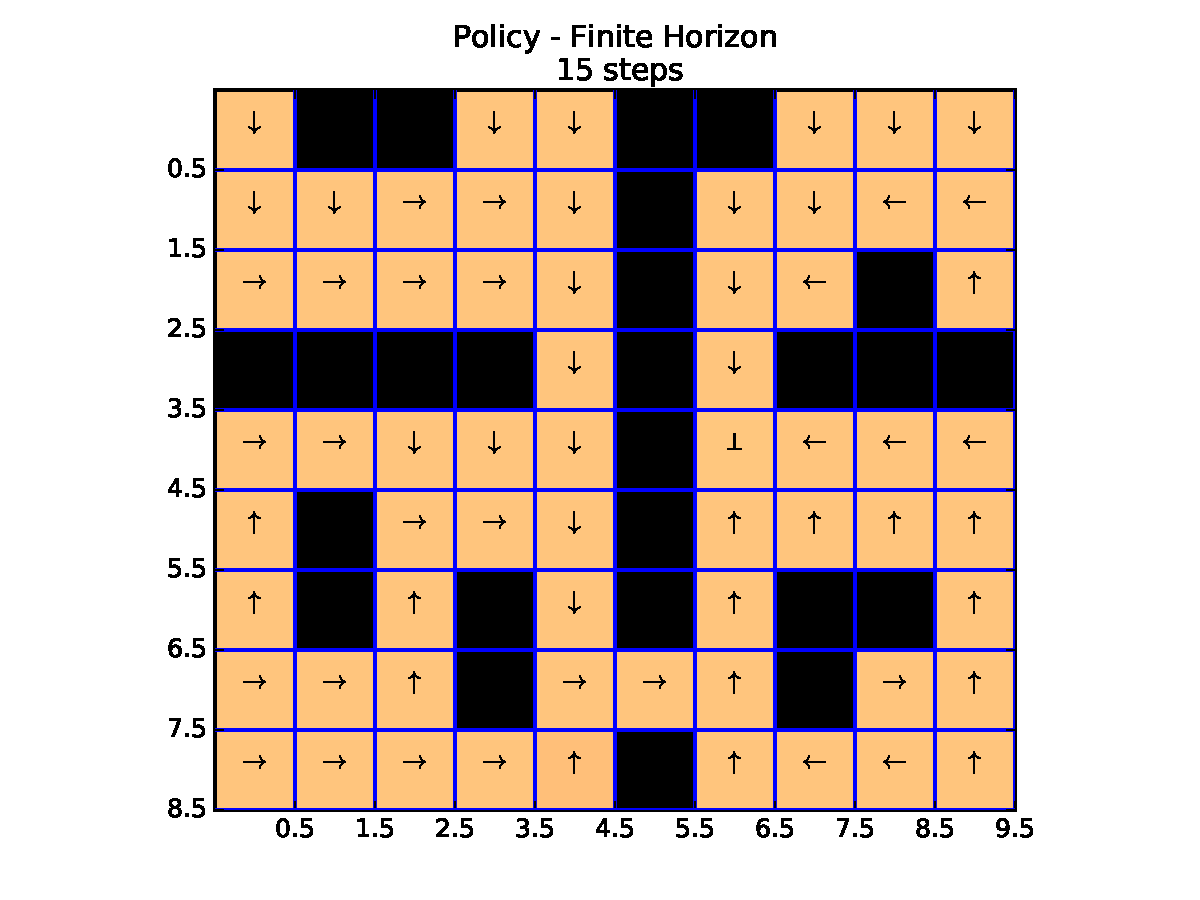
\includegraphics[scale=0.4]{Gridworld/policy_Fin_15.pdf}
	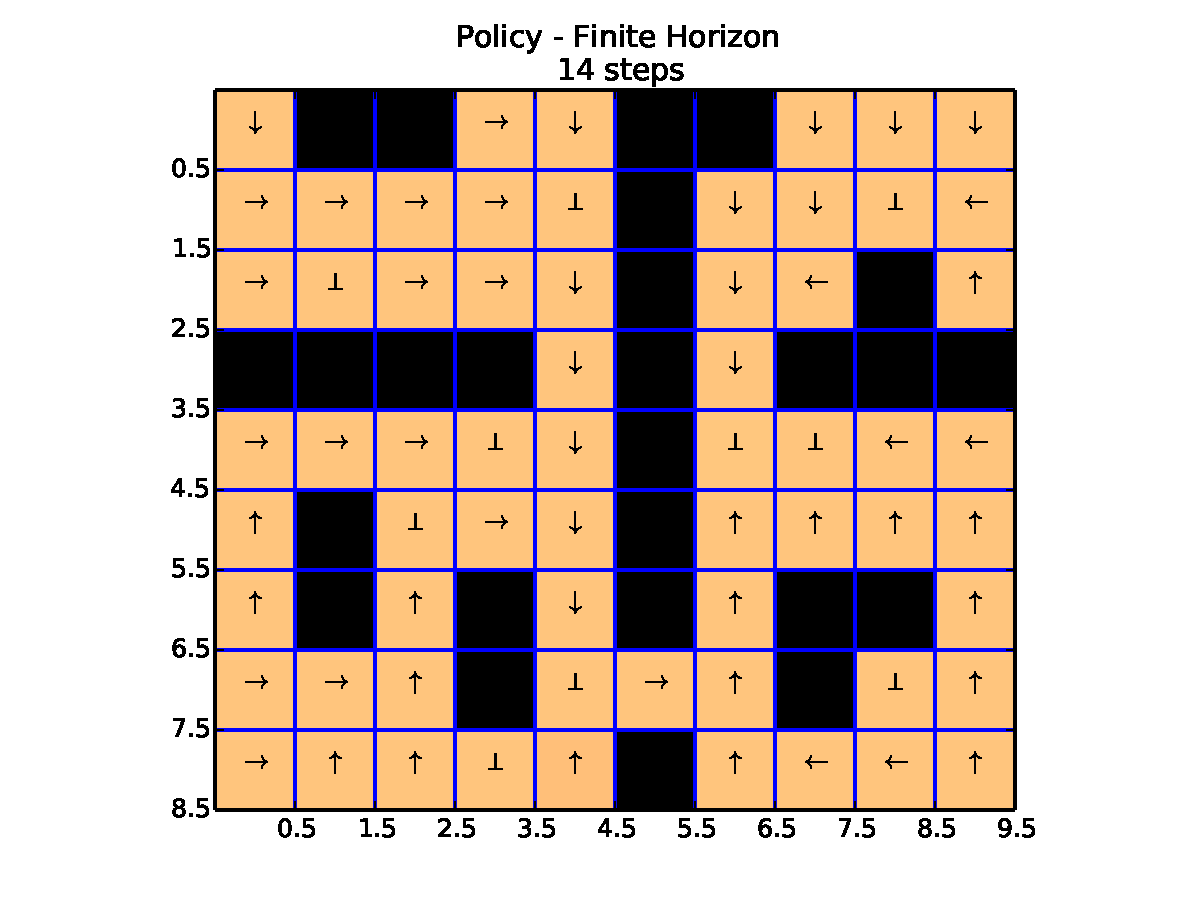
\includegraphics[scale=0.4]{Gridworld/policy_Fin_14.pdf}\\
	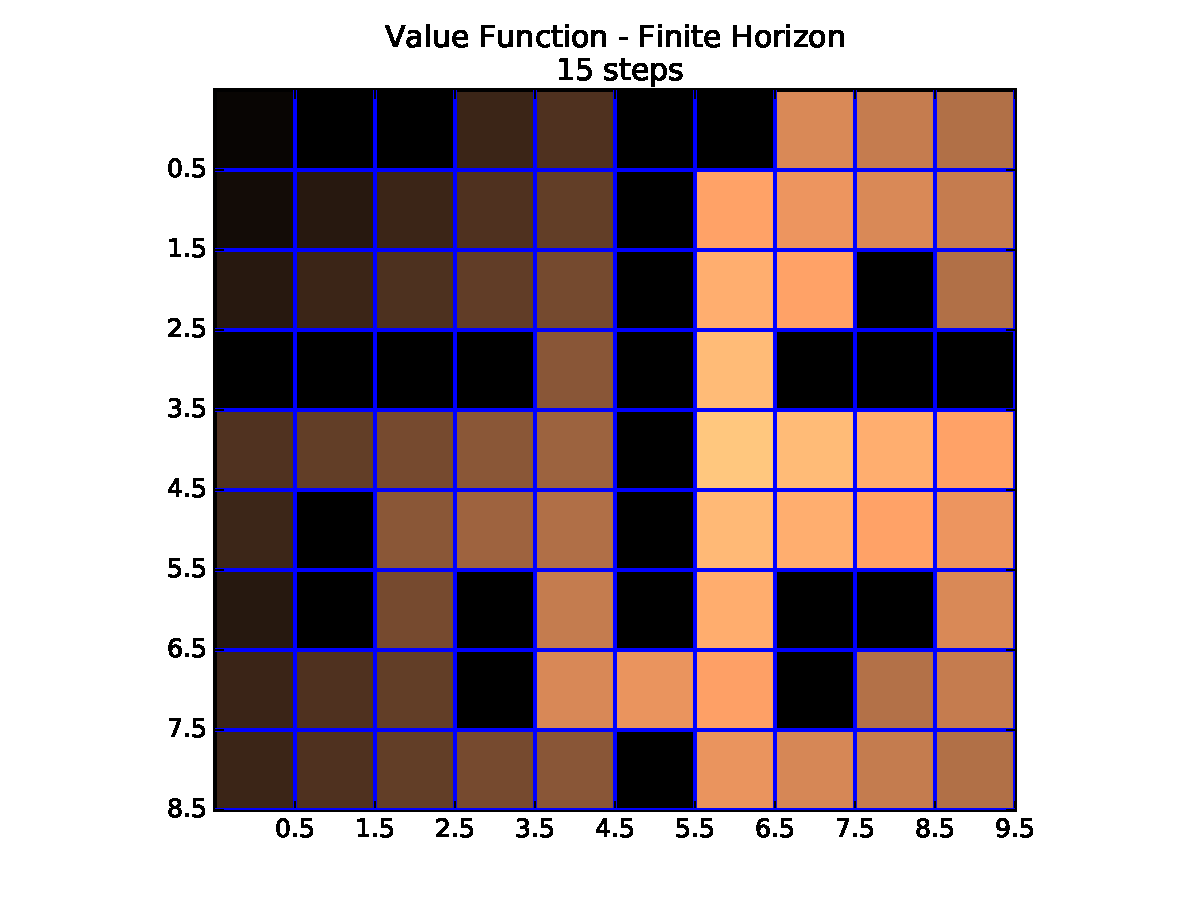
\includegraphics[scale=0.8]{Gridworld/value_Fin_15.pdf} 


	Our policy seems appropriate given our explanation. The robot does collect dirt if it is far enough away from the toy (5,1) but otherwise will prioritize getting towards the toy. It seems so reckless that it even walks over the cat space to get to it when starting in (9,4). This however changes once the robot is limited to 14 steps forcing our robot to simply collect dirt beside the cat in (9,4). 
	\lstinputlisting[language=Python,firstline=23,lastline=23]{Gridworld/gridWorld.py}
	...
	\lstinputlisting[language=Python,firstline=139,lastline=155]{Gridworld/gridWorld.py}
	...
	\lstinputlisting[language=Python,firstline=156,lastline=190]{Gridworld/gridWorld.py}
	...
	\lstinputlisting[language=Python,firstline=193,lastline=217]{Gridworld/gridWorld.py}
	...
\end{answer}

\end{question}

%----------------------------------------------


\begin{question}{Infinite Horizon Problem - Part 1}{4}
We now consider the infinite horizon problem, where $T=\infty$. Rewrite Equation~\eqref{Eq:J} for the infinite horizon case adding a discount factor $\gamma$. Explain briefly why the discount factor is needed.

\begin{answer}
\begin{equation}
	J_\pi = \mathbb{E}_\pi\left[\sum_{t=1}^{\infty} \gamma^{t-1} r_t(s_t,a_t)\right],
	\label{Eq:A}
\end{equation}
Since like above described rewards in our case are independent of
the action and the actions are deterministic, Equation \eqref{Eq:A} becomes
\begin{equation}
	J_\pi = \mathbb{E}_\pi\left[\sum_{t=1}^{\infty} \gamma^{t-1} r_t(s_t)\right],
	\label{Eq:B}
\end{equation}

The discount factor is needed for convergence. Without the discount factor state values would be summed up until infinity. Therefore the discount factor always has to be smaller than 1, because than later summands of \eqref{Eq:B} go against 0, since the coefficient of the rewards are $\gamma^t$, and $\lim\limits_{t\rightarrow\infty}(\gamma^t) = 0$ for $\gamma < 1$ .In addition to that it makes decisions, which are made in the future ,be considered less important than more imminent decisions. The smaller the discount factor is, the faster the algorithm converges.

\end{answer}

\end{question}

%----------------------------------------------


\begin{question}{Infinite Horizon Problem - Part 2}{6}
Calculate the optimal actions with the infinite horizon formulation. Use a discount factor of $\gamma=0.8$ and attach the new policy and value function plots.
What can we say about the new policy? Is it different from the finite horizon scenario? Why?

\begin{answer}
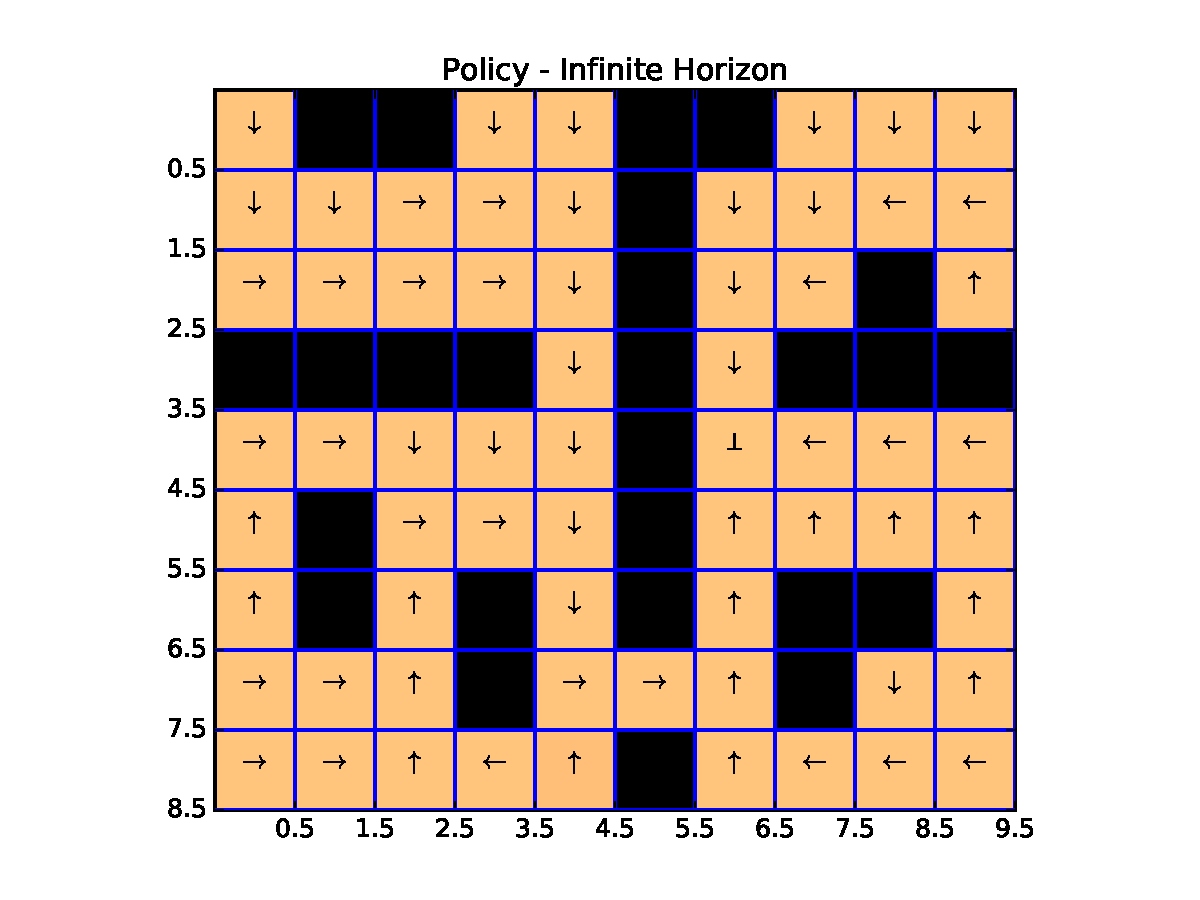
\includegraphics[scale=0.4]{Gridworld/policy_Inf_08.pdf}
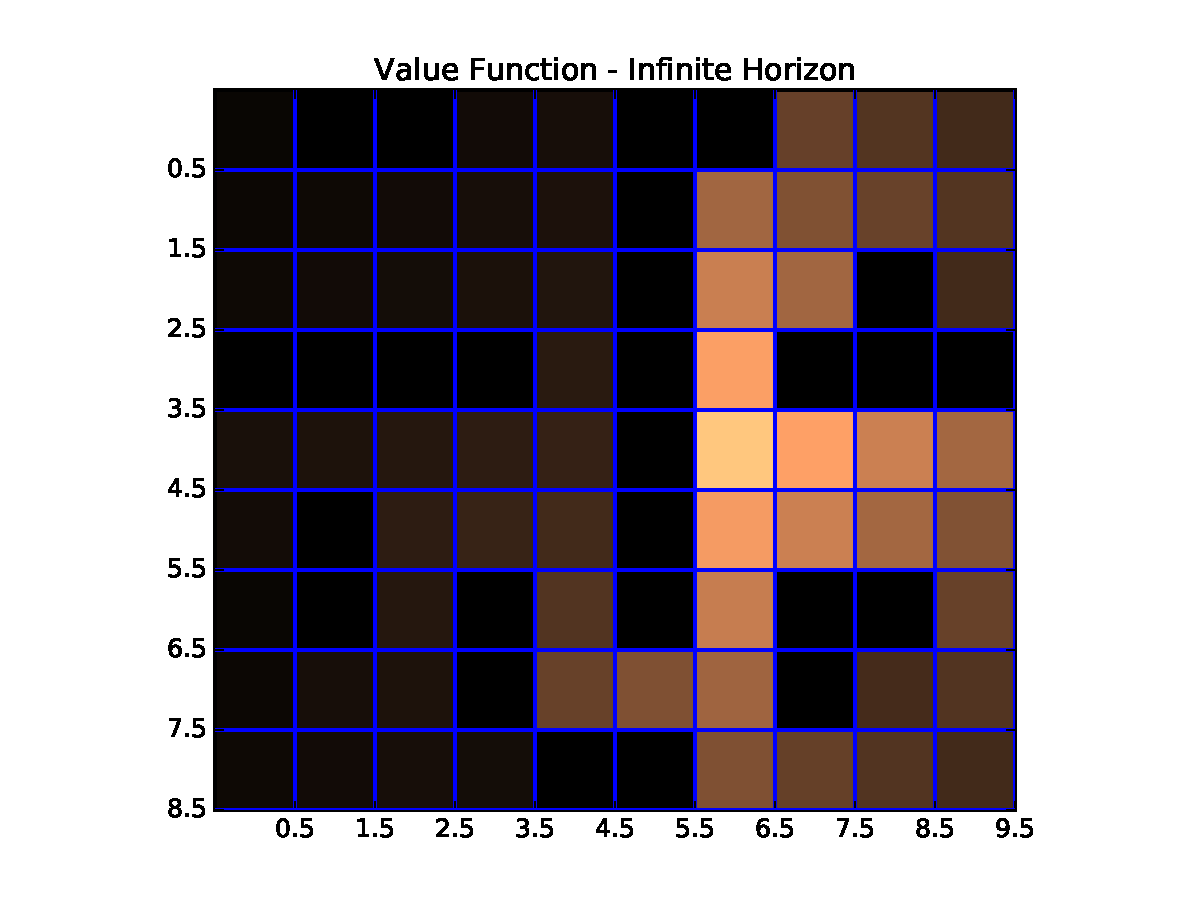
\includegraphics[scale=0.4]{Gridworld/value_Inf_08.pdf}\\

We can say, that it is the optimal policy for the grid world, since iterating the Bellman Equation (Value Iteration) converges to the optimal value function, from which we extracted the optimal policy. It is different, because it decides at (9,4) to rather take the detour instead of passing by the cat. Here we have the optimal policy, the value iteration from a) would need more steps to realize that the route via the cat has a smaller return.\\

\lstinputlisting[language=Python,firstline=36,lastline=36]{Gridworld/gridWorld.py}
	...
	

\end{answer}

\end{question}

%----------------------------------------------


\begin{question}{Finite Horizon Problem with Probabilistic Transition Function}{10}
After a fight with the cat, the robot experiences control problems. 
For each of the actions \textit{up, left, down, right}, the robot has now a probability $0.7$ of correctly performing it and a probability of $0.1$ of performing another action according to the following rule: if the action is \textit{left} or \textit{right}, the robot could perform \textit{up} or \textit{down}. If the action is \textit{up} or \textit{down}, the robot could perform \textit{left} or \textit{right}.
Additionally, the action can fail causing the robot to remain on the same state with probability $0.1$.
Using the finite horizon formulation, calculate the optimal policy and the value function. Use a time horizon of $T=15$ steps as before. Attach your plots and comment them: what is the most common action and why does the learned policy select it?

\begin{answer}

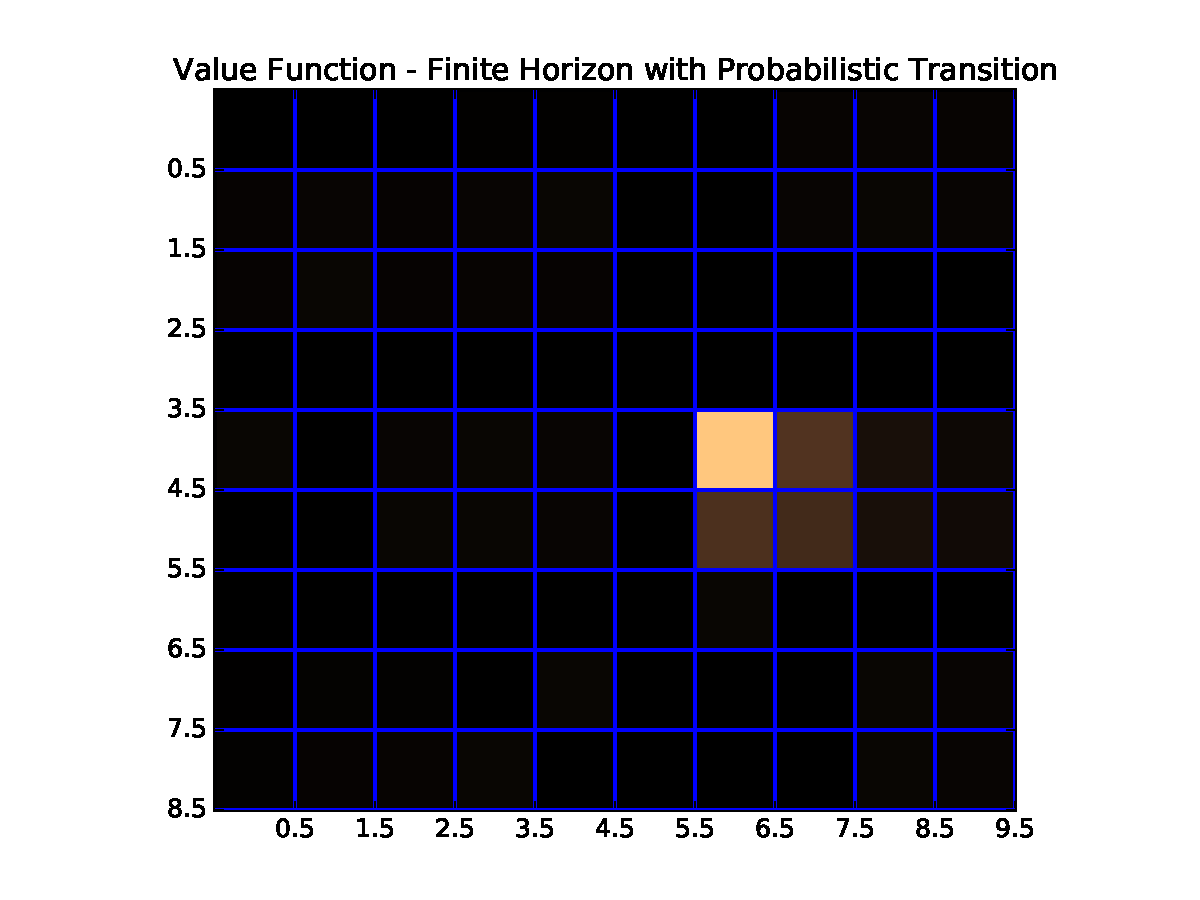
\includegraphics[scale=0.4 ]{Gridworld/value_Fin_15_prob.pdf}
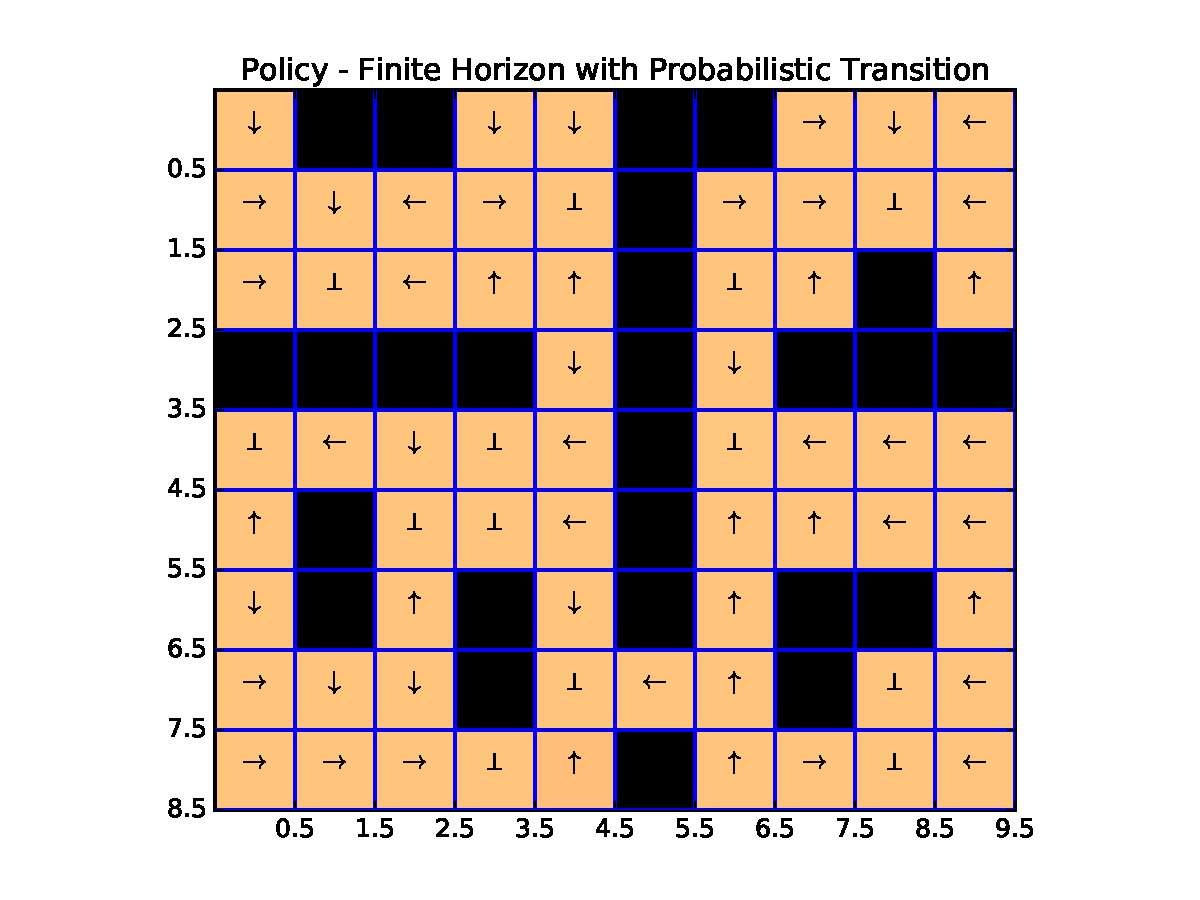
\includegraphics[scale=0.4 ]{Gridworld/policy_Fin_15_prob.pdf}

The fact that the robot can by accident do other actions than expected slows learning tremendous since the negative values of the walls influence other state values. Because of that the most common action the robot chooses is to stay at his position. At all the 'Dirt' postions, the robot rather remains at the Dirt than risking running into a wall.\\
However, if you run the algorithm for longer time, the results become similar to a). For e.g. T=250 we get: \\
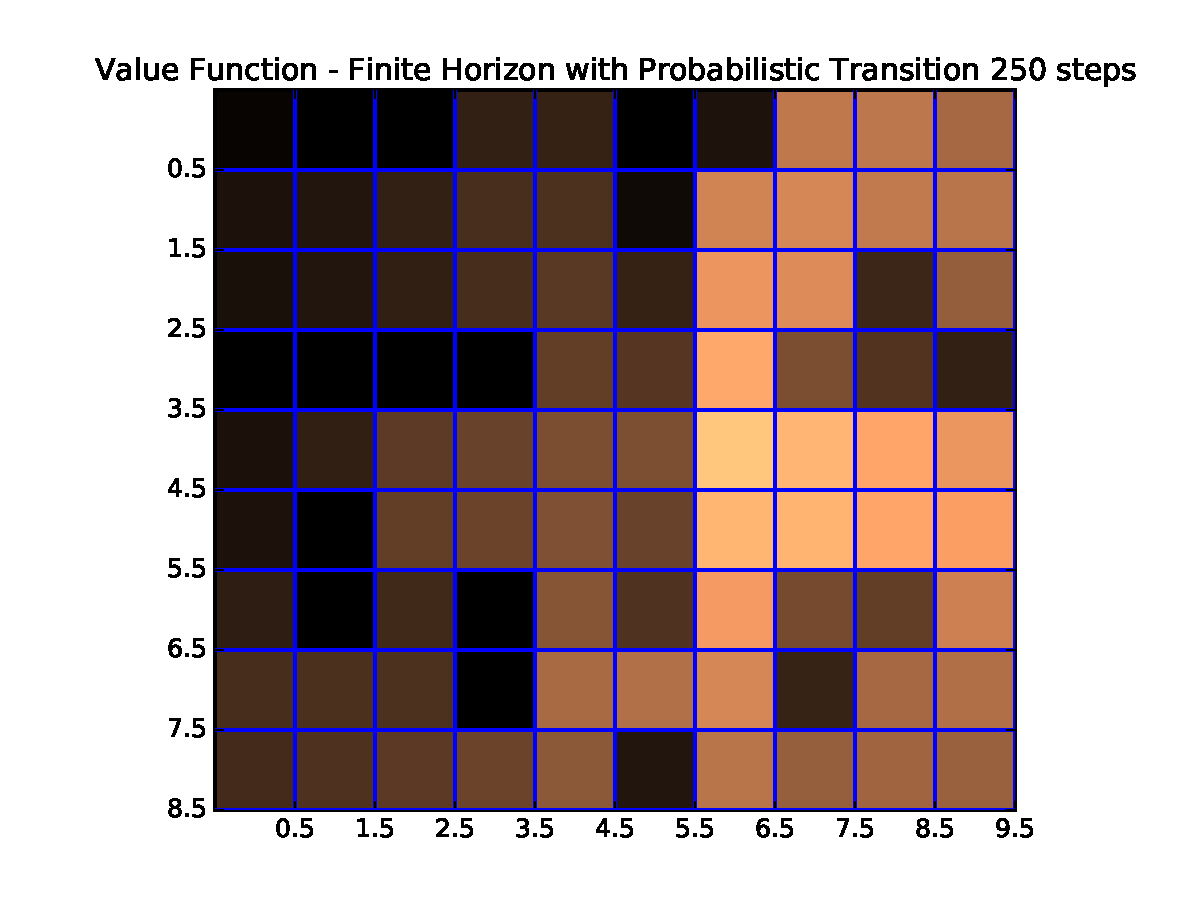
\includegraphics[scale=0.4 ]{Gridworld/value_Fin_15_proof.pdf}
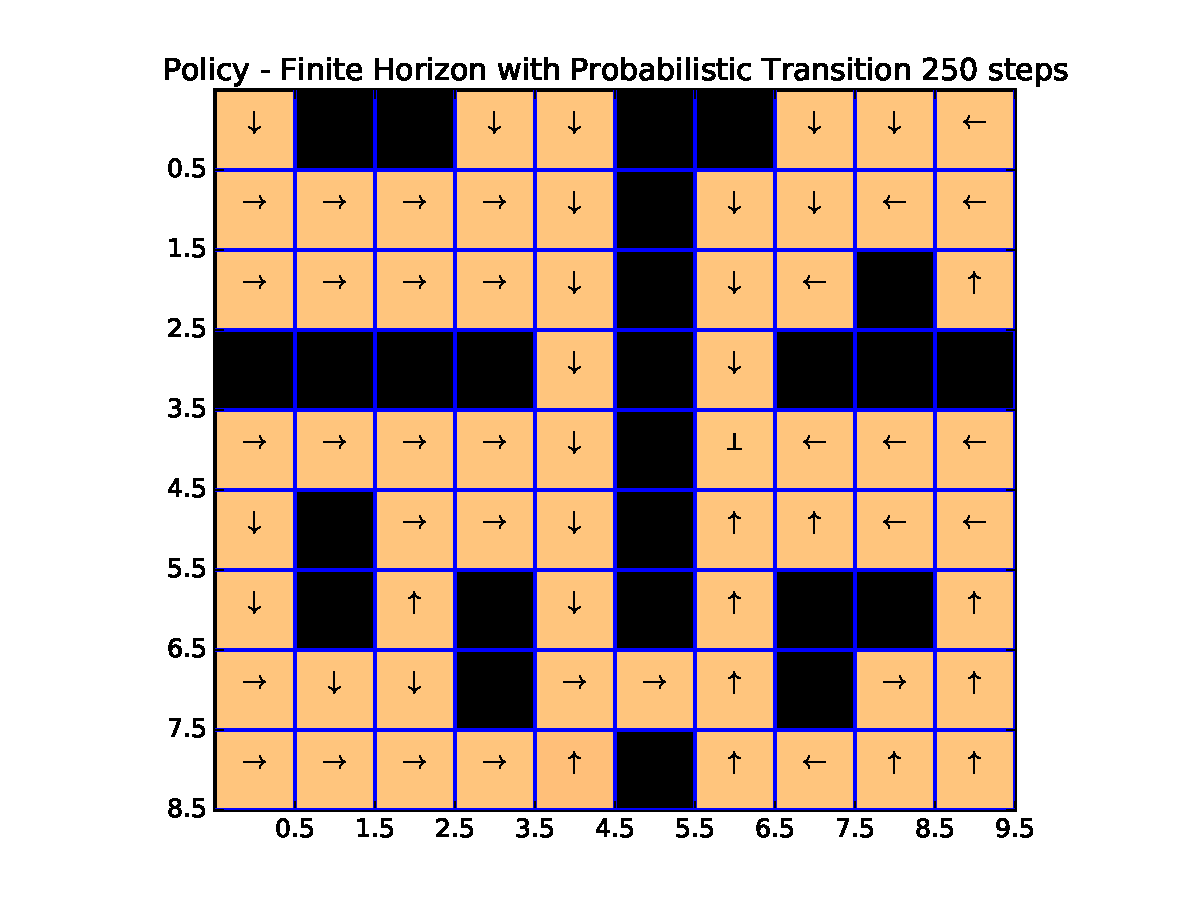
\includegraphics[scale=0.4 ]{Gridworld/policy_Fin_15_proof.pdf}

\lstinputlisting[language=Python,firstline=48,lastline=48]{Gridworld/gridWorld.py}
...

\lstinputlisting[language=Python,firstline=218,lastline=246	]{Gridworld/gridWorld.py}
\end{answer}

\end{question}

%----------------------------------------------


\begin{question}[bonus]{Reinforcement Learning - Other Approaches}{8}
What are the two assumptions that let us use the Value Iteration algorithm? What if they would have been not satisfied? Which other algorithm would you have used? Explain it with your own words and write down its fundamental equation.

\begin{answer}
	The Value Iteration algorithm is based on two fundemental assumptions . The first is, that we know completly our environment and therefore can \textit{compute} the Value function and the associated policy. The second assumption is that its computation doesn't exceed the scale of complexity. That is to say, that we can compute it with the computer.\\ 
	If these assumptions weren't given, we probably would use the \textit{Temporal Difference Learning} algorithm, which doesn't compute the value funtion directly, but approximates it. Through the approximation of the value function we could get our policy. Its fundamental equation is given by the following update rule:\\
	\begin{equation}
		V_{t+1}(s_t) = V_t(s_t) + \alpha[r_{t}+\gamma V_t(s_{t+1})-V_t(s_t)]
	\end{equation}
\end{answer}
\end{question}


\end{questions}


%=========================================================

\end{document}
